\section{Kiến Trúc Tổng Thể và Phục Hồi Cấu Trúc Vật Lý Ấn Bản}

Để xử lý đồng thời các nhiễu vật lý ở đầu vào và những khác biệt ngôn ngữ học giữa hai hệ chữ viết, quy trình xây dựng ngữ liệu được tổ chức thành ba phân vùng xử lý nối tiếp nhau như minh họa ở Hình~\ref{fig:arch}. Trong kiến trúc này, thông tin không chỉ chảy một chiều từ ảnh quét sang văn bản, mà kết quả nhận dạng từ vế Hán Nôm còn được tận dụng ngược lại như một nguồn tiên nghiệm ngữ âm nhằm chọn lọc giữa các giả thuyết nhận dạng Quốc ngữ trước khi hai luồng hội tụ ở bước dóng hàng quy hoạch động hai tầng.

\begin{figure}[H]
    \centering
    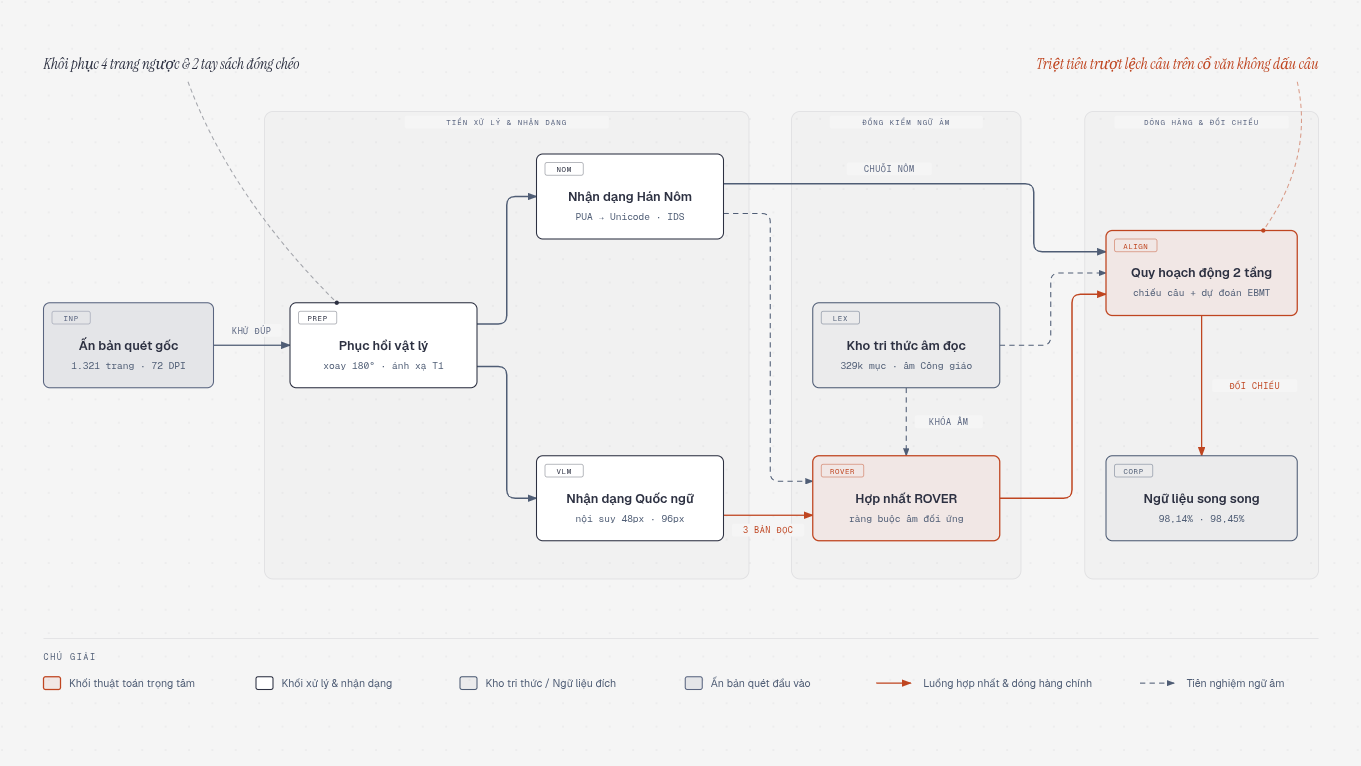
\includegraphics[width=\linewidth]{images/fig1-arch.png}
    \caption{Kiến trúc tổng thể quy trình xây dựng ngữ liệu song song Hán Nôm -- Quốc ngữ từ ấn bản lịch sử}
    \label{fig:arch}
\end{figure}

\subsection{Phân tích mật độ điểm ảnh gốc và trích xuất bảo toàn thông tin}

Trong nhiều quy trình số hóa tài liệu, ảnh trang sách thường được kết xuất ở độ phân giải $300\text{ DPI}$ với kỳ vọng cải thiện độ nét cho mô hình nhận dạng. Tuy nhiên, khi kiểm tra trực tiếp luồng ảnh nhúng bên trong tệp quét gốc của hai tập sách, nhóm ghi nhận các trang ảnh thực chất đã được số hóa ở mật độ xấp xỉ $72\text{ DPI}$, tương ứng với kích thước khoảng $800 \times 1135$ đến $1067 \times 1513$ điểm ảnh. Xét theo nguyên lý lấy mẫu tín hiệu, việc phóng toàn trang lên $300\text{ DPI}$ chỉ tạo ra nội suy phóng đại gấp khoảng $4{,}17$ lần mỗi chiều, làm tăng dung lượng lưu trữ khoảng $5{,}5$ lần mà không bổ sung thêm chi tiết tần số cao thực sự cho bộ nhận dạng toàn trang.

Từ quan sát đó, nhóm quyết định trích xuất ảnh trang ở đúng độ phân giải gốc $72\text{ DPI}$ nhằm giữ nguyên phân bố mức xám ban đầu cho luồng nhận dạng Hán Nôm và tiết kiệm dung lượng lưu trữ. Ở nhánh Quốc ngữ, phép nội suy phóng đại chỉ được áp dụng có chọn lọc ở mức từng dòng chữ đã cắt rời bằng bộ lọc Lanczos bậc cao khi đưa vào mô hình thị giác, nhằm đáp ứng kích thước lưới vi mảnh của bộ mã hóa ảnh mà không làm phình kích thước tập ảnh gốc.

\subsection{Mô hình hóa ánh xạ trang tuyến tính từng đoạn}

Sau khi loại bỏ hai trang quét đúp ở Tập 2 và tách riêng các trang không thuộc chính văn (bìa, lời tựa, mục lục, chú thích và trang trắng), gọi $\mathcal{I}_{\text{vi}}$ và $\mathcal{I}_{\text{ch}}$ lần lượt là tập chỉ số trang chính văn Quốc ngữ và Hán Nôm. Do Tập 1 có trang trắng xen giữa, hai cặp tay sách bị hoán vị và hai trang Quốc ngữ bị quét thiếu, quan hệ ghép trang không thể biểu diễn bằng một công thức tuyến tính đơn lẻ cho cả hai tập, mà được mô hình hóa dưới dạng hàm tuyến tính từng đoạn theo thứ tự đọc xuôi của vế Quốc ngữ và thứ tự đọc ngược của vế Hán Nôm.

Đối với Tập 2 ($683$ trang hiệu lực sau khi loại hai trang trùng thứ $27$ và $28$), cấu trúc đối xứng được duy trì liên tục trên toàn bộ $331$ cặp trang chính văn theo biểu thức:
\begin{equation}
    f_{\text{Tập 2}}(p_{\text{vi}}) = 681 - p_{\text{vi}}, \quad \forall p_{\text{vi}} \in [7, 337].
\end{equation}
Trái lại, trên Tập 1 ($636$ trang), ánh xạ $f_{\text{Tập 1}}: \mathcal{I}_{\text{vi}} \to \mathcal{I}_{\text{ch}}$ cần được phân rã thành bảy miền liên tiếp nhằm phản ánh chính xác hai cặp tay sách đóng chéo và bước nhảy pha $\Delta = -2$ sau hai trang Hán Nôm khuyết vế Quốc ngữ ($p_{\text{ch}} \in \{359, 358\}$):
\begin{equation}
    f_{\text{Tập 1}}(p_{\text{vi}}) =
    \begin{cases}
        635 - p_{\text{vi}}, & p_{\text{vi}} \in [11, 17] \cup [19, 42] \cup [45, 52] \cup [55, 275] \\
        625 - p_{\text{vi}}, & p_{\text{vi}} \in [43, 44] \quad \text{(hoán vị tay sách thứ nhất: } 582, 581\text{)} \\
        645 - p_{\text{vi}}, & p_{\text{vi}} \in [53, 54] \quad \text{(hoán vị tay sách thứ hai: } 592, 591\text{)} \\
        633 - p_{\text{vi}}, & p_{\text{vi}} \in [276, 314] \quad \text{(dịch pha } \Delta = -2 \text{ sau } 2 \text{ trang khuyết).}
    \end{cases}
\end{equation}
Để tránh sai sót thủ công khi khai báo các miền trang, quá trình phân hoạch luôn đi kèm bước kiểm tra tự động ba điều kiện đóng: các nhóm trang không giao nhau và phủ kín khoảng $[1, N_{\text{trang}}]$, tập ảnh xuất hiện ở hai vế của bảng ghép trang trùng khớp với tập trang chính văn, và toàn bộ ảnh sau khi xoay phục hồi $180^\circ$ bốn trang quét ngược đều giữ chiều đứng ($W < H$).

\subsection{Tách vùng chính văn bằng hình thái học và thống kê bền vững}

Đặc điểm chung của các trang in khắc đầu thế kỷ XX là sự hiện diện của khung viền hoa văn kép bao quanh vùng chữ, dòng số trang in ở lề trên trang Quốc ngữ (có dạng \code{- 53 - ( 584 )}) và tên sách kèm số tờ bằng chữ Hán ở mép gáy ngoài khung của trang Nôm. Nếu giữ lại các thành phần rìa này trong chuỗi văn bản đầu vào, chúng sẽ tạo ra sự chênh lệch không có đối ứng giữa hai vế và làm giảm trực tiếp độ tương đồng khi dóng hàng.

Nhằm lọc sạch các nhiễu rìa mà không vô tình xóa mất cột kết đoạn ngắn ở cuối mục, hệ thống áp dụng bộ lọc hình học hai nhánh thích ứng theo kích thước từng trang. Trên trang Hán Nôm, các cột văn bản chuẩn bên trong khung được xác định từ những vùng nhận dạng có độ dài tối thiểu $8$ ký tự, từ đó ước lượng biên bao $[x_{\min}, x_{\max}] \times [y_{\min}, y_{\max}]$ cùng trung vị độ rộng cột $\tilde{w} = \operatorname{median}_k(w_k)$. Một khung hộp có tâm $(x_c, y_c)$ và kích thước $(w, h)$ sẽ bị loại nếu nằm ngoài lề ngang với dung sai bất đối xứng về bên trái ($x_c < x_{\min} - 1{,}45\tilde{w}$ nhằm giữ lại cột ngắn kết thúc đoạn theo chiều đọc phải sang trái, hoặc $x_c > x_{\max} + 0{,}8\tilde{w}$ ở lề phải), vượt quá biên dọc $y_c \notin [y_{\min} - 0{,}5\tilde{w},\; y_{\max} + 0{,}5\tilde{w}]$, quá mảnh như đoạn đường kẻ khung bị nhận nhầm ($w < 0{,}48\tilde{w}$), hoặc là nhiễu đơn tự kéo dài bất thường ($|\text{chuỗi}| = 1$ và $h / w > 3{,}5$). Tương tự, trên trang Quốc ngữ, đỉnh vùng thân trang $y_{\text{body}}$ được ước lượng từ cực tiểu tung độ của các dòng văn bản thông thường (có ít nhất $15$ ký tự), cho phép tách bỏ có chọn lọc các dòng tiêu đề số trang nằm tách biệt phía trên trước khi ghép dòng.

\begin{softbox}
\textbf{Nhận xét kỹ thuật:} Việc sử dụng trung vị độ rộng cột $\tilde{w}$ thay cho giá trị trung bình giúp các ngưỡng lọc ít bị ảnh hưởng bởi những khung hộp ngoại lai (chẳng hạn hai cột chập dính vào nhau hoặc vết chấm mực ở mép giấy), đồng thời giữ tính ổn định khi tỷ lệ kích thước ảnh thay đổi giữa các trang quét.
\end{softbox}
